\documentclass[a4paper,12pt]{article}

\usepackage[T2A]{fontenc}
\usepackage[utf8]{inputenc}
\usepackage[english, russian]{babel}

\usepackage{amsmath}
\usepackage{mathtools}
\usepackage{cmap}
\usepackage{xcolor}
\usepackage{graphicx}
\usepackage{float}
\usepackage{listings}
\usepackage{hyperref}
\usepackage{shorttoc}
\usepackage{caption}


% Пути к изображениям (предполагается, что изображения находятся в папке 'img')
\graphicspath{{./img/}}

% Настройка гиперссылок
\definecolor{linkcolor}{HTML}{000000}
\definecolor{urlcolor}{HTML}{0085FF}
\hypersetup{
    pdfstartview=FitH,
    linkcolor=linkcolor,
    urlcolor=urlcolor,
    colorlinks=true
}

% Настройка окружения для округлых скобок
\DeclarePairedDelimiter{\floor}{\lfloor}{\rfloor}

% Переименование содержания
\renewcommand*\contentsname{Содержание}

% Настройки для листингов кода
\lstset{
    basicstyle=\small\ttfamily,
    breaklines=true,
    frame=single,
    numbers=none, % Отключение номеров строк
    showstringspaces=false,
    keywordstyle=\color{blue},
    commentstyle=\color{green!50!black},
    stringstyle=\color{red},
    captionpos=b
}

% Команда для вставки рисунков
\newcommand{\plot}[3]{
    \begin{figure}[H]
        \centering
        \includegraphics[width=0.7\textwidth]{#1.png}
        \caption{#2}
        \label{#3}
    \end{figure}
}

\begin{document}

\begin{titlepage}
    \begin{center}
        {\large Санкт-Петербургский политехнический университет\\Петра Великого}
    \end{center}
    
    \begin{center}
        {\large Физико-механический институт}
    \end{center}
    
    \vspace{8em}
    
    \begin{center}
        {\bfseries Отчёт по лабораторной работе №3:\\ ``Ситуативные сети''}
    \end{center}
    
    \vspace{4em}
     
    \begin{flushleft}
        \hspace{22em}Выполнил студент:\\
        \hspace{22em}Завьялов В. В.\\
        \hspace{22em}группа: 5040102/30201
        
        \vspace{2em}
        
        \hspace{22em}Проверил:\\
        \hspace{22em}к.ф.-м.н., доцент\\
        \hspace{22em}Баженов А. Н.
    \end{flushleft}
    
    \vspace{12em}
    
    \begin{center}
        Санкт-Петербург\\2025 г.
    \end{center}
    
\end{titlepage}

\tableofcontents

\newpage

\section{Постановка задачи}
Необходимо реализовать протоколы OSPF и Selective Repeat в сети из набора маршрутизаторов, случайно расположенных в двумерном пространстве. Требуется обеспечить надёжную доставку пакетов от источника (router с индексом 0) к получателю (router с индексом 1), используя два независимых механизма:

\begin{itemize}
    \item Протокол маршрутизации OSPF (Open Shortest Path First), определяющий кратчайший путь между узлами сети (маршрутизаторами).
    \item Протокол надёжной передачи на основе скользящего окна Selective Repeat, который позволяет восстанавливать утраченные в сети пакеты и контролировать корректную доставку.
\end{itemize}

Дополнительно модель учитывает возможность отказа отдельных узлов (маршрутизаторов) с некоторой вероятностью и их последующего восстановления.

\section{Теория}

\subsection{Open Shortest Path First}

Протокол OSPF (Open Shortest Path First) является одним из наиболее широко применяемых протоколов внутренней маршрутизации (IGP) в современных IP-сетях. Он основан на принципе протокола состояния каналов (Link State Protocol), предполагающем обмен информацией о текущем состоянии всех каналов между маршрутизаторами внутри одной автономной системы. В отличие от протоколов, ориентированных на дистанционно-векторный подход, OSPF поддерживает точное знание глобальной структуры сети, а не ограничивается информацией о соседях или кратчайших дистанциях до определённых подсетей.

Основой работы OSPF является построение всеобъемлющей карты сети, одинаковой на всех маршрутизаторах. Каждый маршрутизатор периодически и при изменениях в топологии рассылает специализированные объявления о состоянии каналов (LSA). На их основе строится единое представление о структуре сети, что обеспечивает маршрутизаторам информацию обо всех доступных узлах и связях между ними. После формирования топологии для каждого узла запускается алгоритм SPF (Shortest Path First), основанный на методе Дейкстры. Этот алгоритм вычисляет кратчайшие пути до всех доступных узлов, учитывая метрики каналов и их состояние. В результате каждый маршрутизатор получает собственную таблицу маршрутизации, которая обеспечивает оптимальную доставку пакетов.

\subsection{Selective Repeat}

\textbf{Selective Repeat} — это протокол надёжной передачи данных, использующий механизм скользящего окна. Он обеспечивает повторную отправку только тех пакетов, которые были потеряны или повреждены, в отличие от более простых протоколов (например, Go-Back-N), где при ошибке необходимо повторно отсылать всю серию пакетов.

Каждая сторона (отправитель и получатель) поддерживает буфер принятых и не подтверждённых (ACK) данных. При получении подтверждения отправитель двигает «окно» и может передавать следующие пакеты. Такое избирательное повторение позволяет эффективнее использовать пропускную способность сети.

\subsection{Отказы и восстановления}

Модель учитывает случайные отказы маршрутизаторов с заданной вероятностью (\texttt{removal\_probability}) и их последующее восстановление (\texttt{recovery\_probability}). При отказе узел перестаёт участвовать в передаче пакетов, а при восстановлении автоматически подключается обратно к сети.

Эти процессы позволяют проверять устойчивость методов маршрутизации и надёжной доставки в постоянно изменяющихся условиях.


\section{Результаты}

\subsection{Нахождение кратчайшего пути}

В ходе симуляции OSPF регулярно пересчитывает кратчайшие пути в сети. При отказе любого маршрутизатора (кроме источника и получателя) пути могут перестраиваться, чтобы обойти сломанный узел. При восстановлении маршрутизатора он снова учитывается в возможных маршрутах. На рисунках 1 и 2 проведена демонстрация работы программы.

\begin{figure}[H]
    \centering
    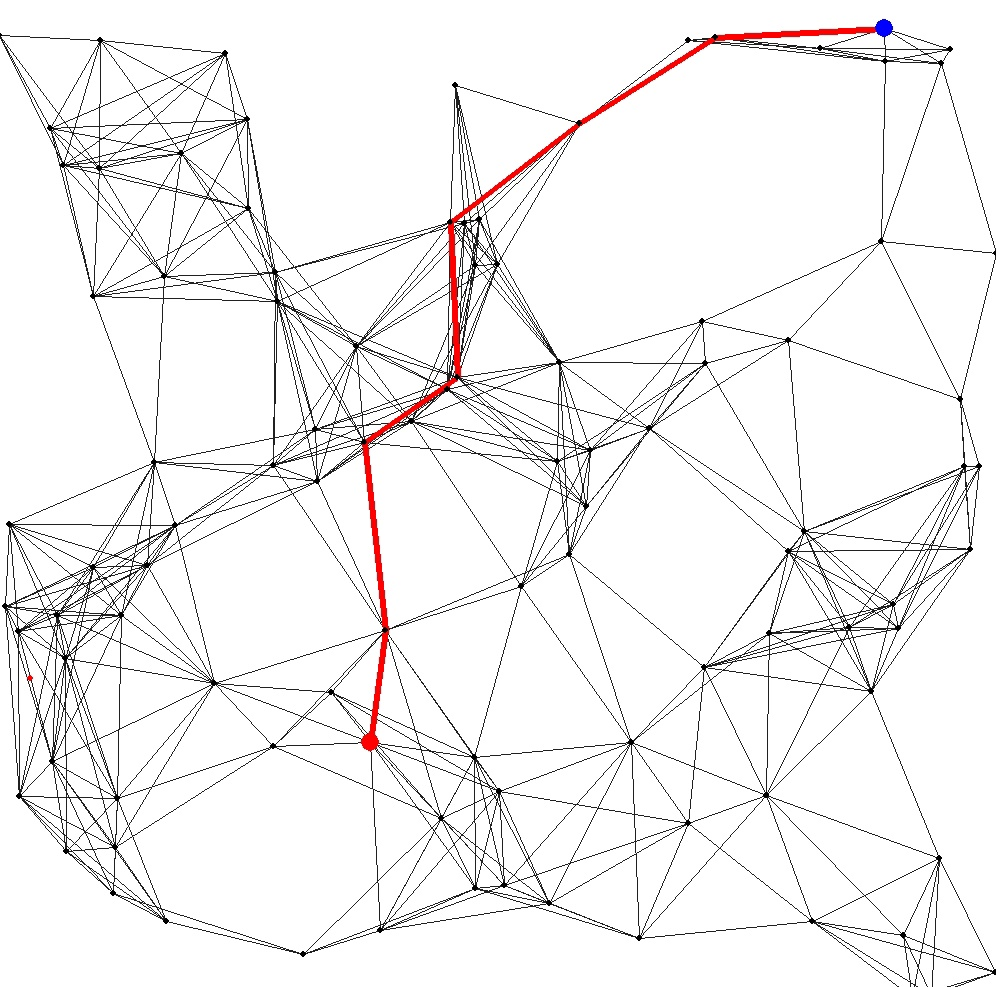
\includegraphics[width=0.8\textwidth]{1.jpg}
    \caption{Демонстрация работы программы}
\end{figure}

\begin{figure}[H]
    \centering
    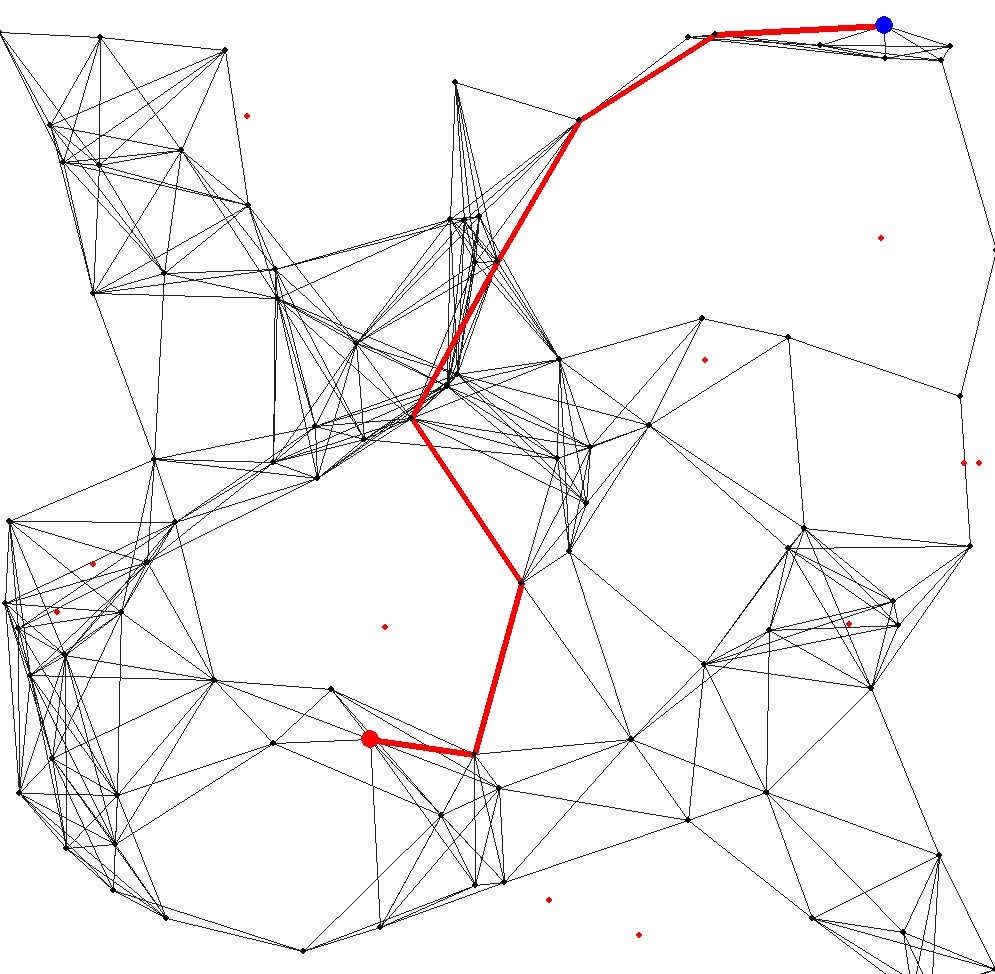
\includegraphics[width=0.8\textwidth]{2.jpg}
    \caption{Выход из строя узлов}
\end{figure}


\subsection{Передача данных с Selective Repeat}

При наличии действующего пути протокол \textbf{Selective Repeat} обеспечивает надёжную доставку данных от источника к получателю.

Если путь остаётся неизменным, пакеты передаются непрерывно. Если же при сбоях маршрут меняется, отправитель корректирует логику передачи (при необходимости перезапускается объект потоковой передачи), и процесс доставки продолжается по новому пути.

\subsection{Анализ устойчивости}

При умеренных значениях вероятности отказа и восстановления сети большинство пакетов успешно достигает пункта назначения, поскольку OSPF и \textbf{Selective Repeat} совместно эффективно адаптируются к изменениям топологии.

\section{Приложения}

Репозиторий с кодом программы и кодом отчета: https://github.com/Nochoooo/networks

\end{document}